%\documentclass[9pt]{elife}
\documentclass[multi=figure,9pt]{standalone}
\usepackage{graphicx}

\RequirePackage[T1]{fontenc}
\RequirePackage[utf8]{inputenc}
\RequirePackage{stix}
\RequirePackage[default]{opensans}
\renewcommand{\ttdefault}{lmtt}

\RequirePackage{microtype}

% Trueno/Open Sans requires a bigger "single" linespread.
\linespread{1.2}
\if@onehalfspacing\linespread{1.5}\fi
\if@doublespacing\linespread{2.0}\fi

\setlength{\abovecaptionskip}{0pt}

\RequirePackage{graphicx,xcolor}
\definecolor{eLifeDarkBlue}{HTML}{273B81}
\definecolor{eLifeLightBlue}{HTML}{0A9DD9}
\definecolor{eLifeMediumGrey}{HTML}{6D6E70}
\definecolor{eLifeLightGrey}{HTML}{929497}

\RequirePackage{booktabs}
\RequirePackage{authblk}

\RequirePackage{changepage}

\RequirePackage{silence}
\WarningFilter{caption}{The option `hypcap=true' will be ignored}

\RequirePackage[labelfont={bf},%
                labelsep=period,%
                justification=raggedright,%
                singlelinecheck=false,%
                skip=0pt,tableposition=top,font={color=eLifeDarkBlue,footnotesize}]
                {caption}

\makeatletter
\renewenvironment{figure}%
{\def\@captype{figure}%
\minipage{\textwidth}}%
{\endminipage}
\makeatother

\let\efloatseparator=\empty

\usepackage{subcaption}

\begin{document}

\begin{figure}
    \centering
    \captionsetup[subfigure]{skip=0pt,font={color=eLifeDarkBlue,footnotesize}}
    \begin{subfigure}[b]{0.9\textwidth}
            \centering
           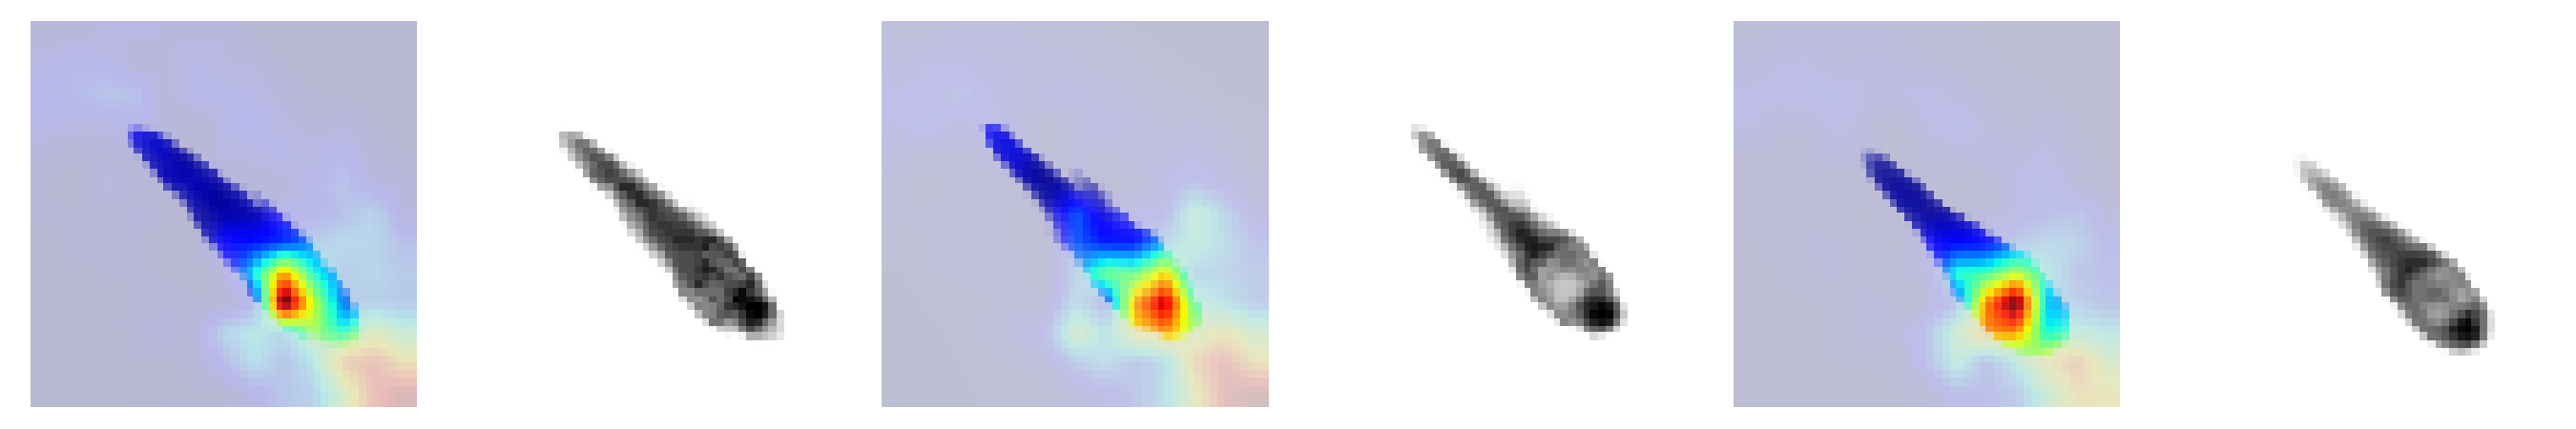
\includegraphics[width=\textwidth]{activations15locusts1h.pdf}
            \caption{Locusts from video 9 with 15 tagged individuals (N: 5101, 7942, 9974) -- the only video with physical tags. The network activates more strongly in regions close to the tag, as well as the bottom right corner.
            }
            \label{fig:activate_locusts}
    \end{subfigure}
    \begin{subfigure}[b]{0.9\textwidth}
           \centering
           	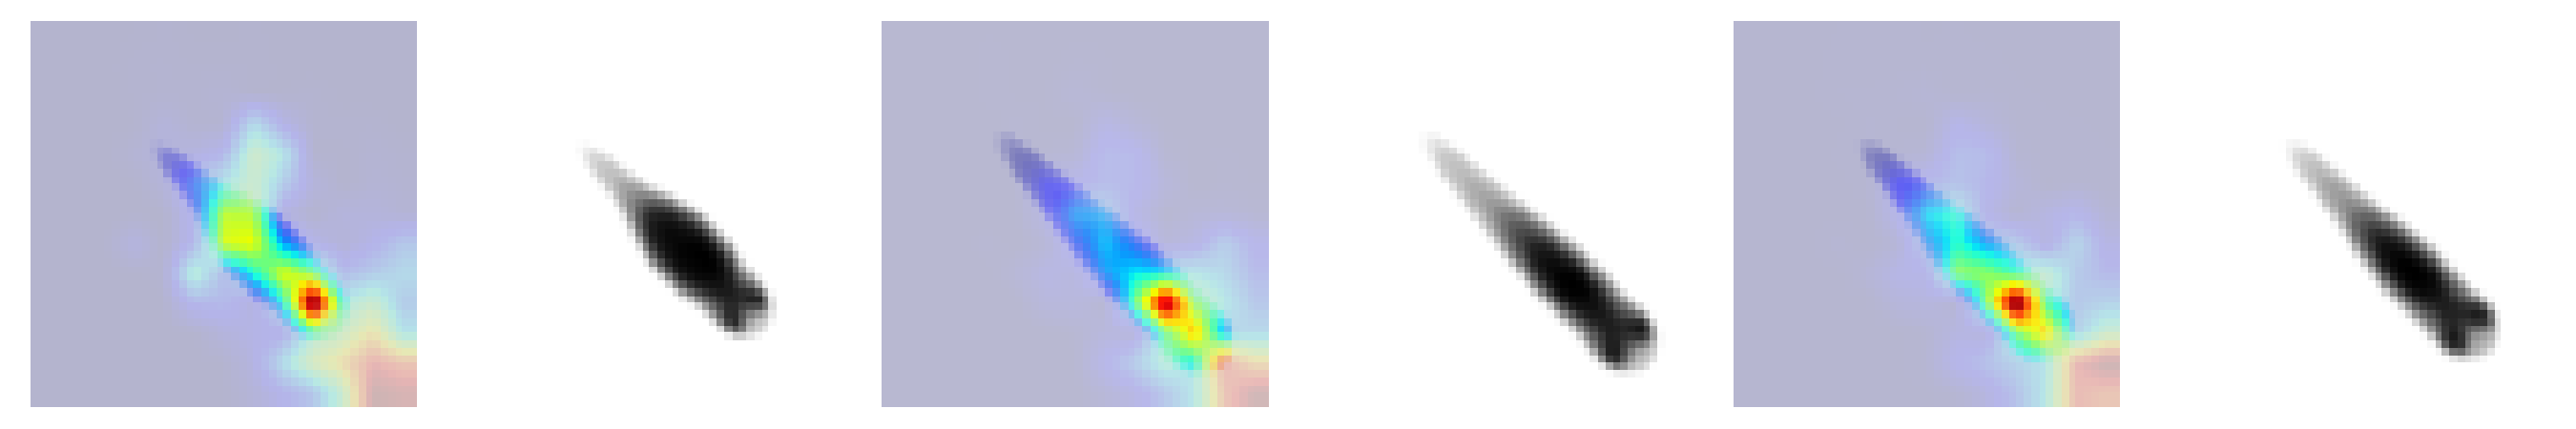
\includegraphics[width=\textwidth]{activationsguppy_8_t36_d15_20191212_085800.pdf}
            \caption{Guppies from video 15 (N: 46378, 34733, 34745). Activations are less focussed and less consistent across individuals.}
            \label{fig:activate_guppies}
    \end{subfigure}
    \begin{subfigure}[b]{0.9\textwidth}
            \centering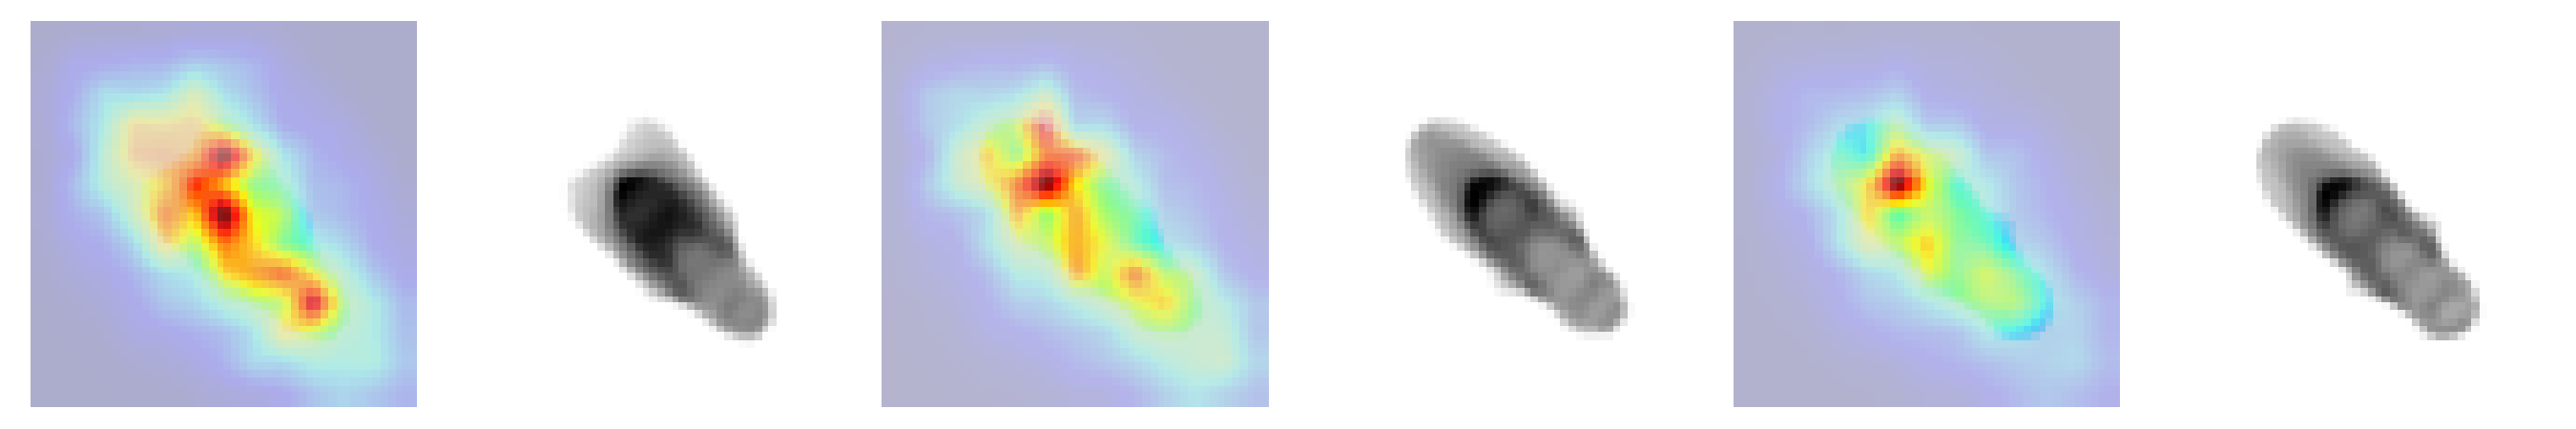
\includegraphics[width=\textwidth]{activationsflies_N59.pdf}
            \caption{Flies from video 8 (N: 993, 1986, 993). Activations are not similar between individuals and show various "hotspots" across the entire body.}
            \label{fig:activate_flies}
    \end{subfigure}
    \begin{subfigure}[b]{0.9\textwidth}
            \centering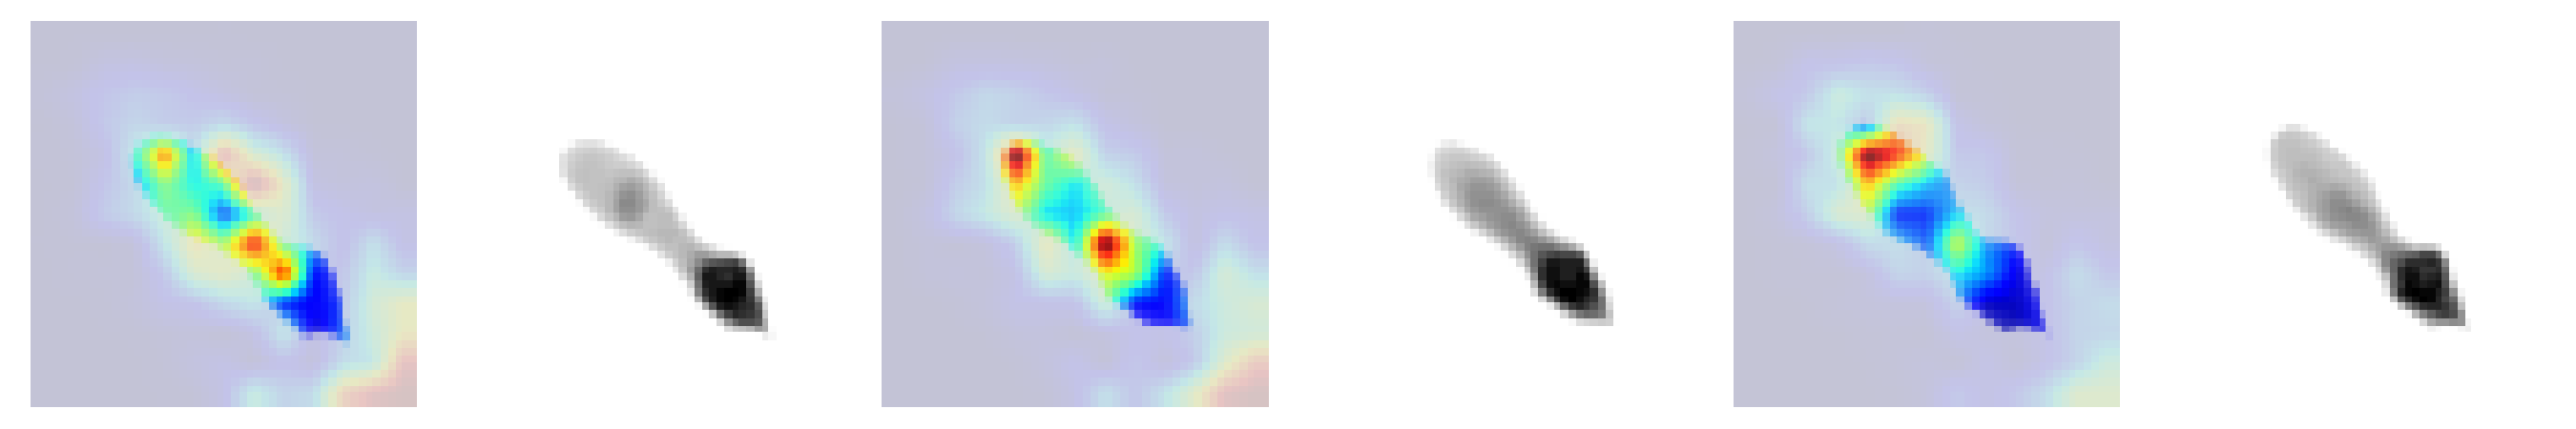
\includegraphics[width=\textwidth]{activationsN05HHS2019-10S-V1.pdf}
            \caption{Termites from video 10 (N: 27097, 31135, 22746). Here, the connections between body-segments show strong activations -- in contrast to very weak ones in other parts of the body. %Anecdotally, but as can be seen here for the first two individuals, activations seem to be strong especially close to connections of body-segments.
            }
            \label{fig:activate_termites}
    \end{subfigure}
\end{figure}

\end{document}